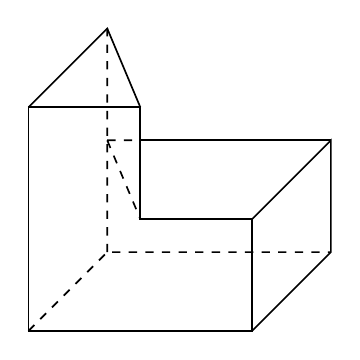
\begin{tikzpicture}[line width=.6pt]
\coordinate (A1) at (0,0);
\coordinate (A2) at (2.84,0);
\coordinate (A3) at (2.84,1.42);
\coordinate (A4) at (1.42,1.42);
\coordinate (A5) at (1.42,2.84);
\coordinate (A6) at (0,2.84);
\coordinate (H) at (1,1);
\coordinate (H1) at (1,2.42);
\coordinate (B2) at (3.84,1);
\coordinate (B3) at (3.84,2.42);
\coordinate (B6) at (1,3.84);
\draw (A1)--(A2)--(A3)--(A4)--(A5)--(A6)--cycle;
\draw (A2)--(B2)--(B3)--(A3);
\draw[dashed] (A1)--(H)--(B2) (H)--(B6);
\draw (A6)--(B6)--(A5);
\draw (B3)--(1.42,2.42);
\draw[dashed] (H1)--(1.42,2.42) (H1)--(A4);
\end{tikzpicture}
